\newpage
\hypertarget{sec:breakpoints}{}
\section{Integrator Breakpoints}
\genHeader

When we introduced the integrator in \hyperlink{sec:app_integrator}{Part 6}, we showed you how it could be used to proceed through your transformation
incrementally. It shows the start point, possible rule candidates, and rule execution for every element the transformation triple. As you saw, this process is
great for a small transformation with only a few objects and rules as it doesn't take that long to run from start to finish. But what if you had a
transformation with 1000 objects, or 100 rules, and suspected there may be an error? As you can imagine, it could potentially take a long time to find a
specific process or repeated execution.

Luckily, this visualized debugger is also able to implement a breakpoint model to pause the execution at any place! We extended our transformation in
the previous section with two rules able to handle partitions, so let's try implementing a breakpoint to pause the process before one of them is executed.

\begin{itemize}

\item[$\blacktriangleright$] You may have noticed when you ran the integrator for the first time that a new \texttt{BreakPointSet.xmi} file was created in
``instances/.'' Double-click this model, expand the tree, and create a new breakpoint (Fig.~\ref{eclipse:breakpointChild}).

\begin{figure}[htbp]
\begin{center}
  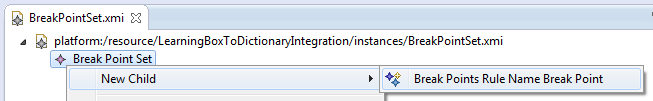
\includegraphics[width=\textwidth]{eclipse_breakpointChild}
  \caption{stuff}
  \label{eclipse:breakpointChild}
\end{center}
\end{figure}

\item[$\blacktriangleright$] Edit its \texttt{Rule Name} property below the editor to \texttt{AllOtherCardsRule} (Fig.~\ref{eclipse:bpProps}).\footnote{Be sure
there are no mistakes in the spelling} This will pause the transformation before it applies this rule. Save the file.

\begin{figure}[htbp]
\begin{center}
  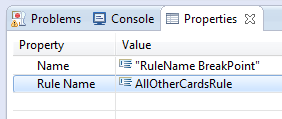
\includegraphics[width=0.5\textwidth]{eclipse_breakpointProperties}
  \caption{stuff}
  \label{eclipse:bpProps}
\end{center}
\end{figure}

\item[$\blacktriangleright$] Right-click on \texttt{corr\_FWD}, start the integrator, and drag-and-drop the breakpoint model into the main window. A small
message should appear confirming that it is setting breakpoints. 

\item[$\blacktriangleright$] Finally, drag \texttt{protocol\_FWD} into the same window. You are now able to quickly skip between breakpoints by pressing
\texttt{alt+shift+ctrl+RIGHT}, or backwards with \texttt{alt+shift+ctrl+LEFT}.

\end{itemize}

Please note that this particular breakpoint model will not stop the integrator if used on \texttt{corr\_BWD}. \texttt{AllOtherCardsRule} was only built to
operate on the source \texttt{Box} model, which means it will never be a valid candidate when transforming from \texttt{Dictionary}. Try experimenting with
\texttt{BoxToDictionaryRule} to see the single breakpoint model work in both directions.
